%%%%%%%%%%%%%%%%%%%%%%%%%%%%%%%%%%%%%%%%%%%%%%%%%%%%%%%%%%%%%%%%%%%%%%
% How to use writeLaTeX: 
%
% You edit the source code here on the left, and the preview on the
% right shows you the result within a few seconds.
%
% Bookmark this page and share the URL with your co-authors. They can
% edit at the same time!
%
% You can upload figures, bibliographies, custom classes and
% styles using the files menu.
%
%%%%%%%%%%%%%%%%%%%%%%%%%%%%%%%%%%%%%%%%%%%%%%%%%%%%%%%%%%%%%%%%%%%%%%

\documentclass[12pt]{article}

\usepackage{float}
\usepackage{sbc-template}
\usepackage{amssymb}
\usepackage{graphicx,url}
\usepackage{hyperref}

%\usepackage[brazil]{babel}   
\usepackage[utf8]{inputenc}  

     
\sloppy

\title{Estudo de técnicas evolutivas de refinamento de parametros de um modelo de automato celular de simulação de incêndio}

\author{Heitor F. Ferreira, Henrique Macarini, Luis G. Seiji Tateishi}


\address{Universidade Federal de Uberlândia (UFU) -- Uberlândia-MG -- Brasil}

\begin{document}

\maketitle

\begin{abstract}
    This work investigates the effectiveness of various evolutionary approaches in enhancing the transition rules in a fire simulation model, utilizing cellular automata. Among the evolutionary methods applied, the evolutionary strategy and the genetic algorithm stand out, the latter using chromosomes in the \(\mathbb{R}^n\) space.
\end{abstract}

\begin{resumo}
    Este trabalho analisa a capacidade de várias abordagens evolutivas em aprimorar as regras de transição em um modelo de simulação de incêndios, empregando autômatos celulares. Entre as metodologias evolutivas aplicadas, destacam-se a estratégia evolutiva e o algoritmo genético, este último utilizando cromossomos no espaço \(\mathbb{R}^n\).
\end{resumo}


\section{Introdução}
Visto que os incêndios florestais tendem a crescer em quantidade com o agravamento dos problemas climaticos, é importante a criação de um modelo capaz de prever com um alto grau de precisão como será a evolução das chamas, logo, a utilização de modelos de otimização

\section{Referencial teórico} \label{sec:firstpage}
O estudo de técnicas evolutivas para o refinamento de parâmetros em modelos de autômatos celulares (CA) de simulação de incêndios tem se destacado como uma área de pesquisa em constante desenvolvimento. Os autômatos celulares oferecem uma abordagem poderosa para modelar a propagação de incêndios, devido à sua capacidade de capturar a dinâmica espacial e temporal do fenômeno.
Nesse contexto, os modelos de CA têm sido amplamente explorados, com destaque para aqueles que buscam simular a propagação de incêndios em diferentes cenários, como florestas heterogêneas e áreas urbanas. A utilização de algoritmos evolutivos, como os algoritmos genéticos, tem se mostrado promissora para ajustar os parâmetros desses modelos como demonstrado em \cite{shan2008genetic}, considerando variáveis como tipo de vegetação, densidade, topografia e direção do vento.
Estudos recentes têm focado não apenas no desenvolvimento de modelos mais precisos, mas também na avaliação do desempenho e validade desses modelos em cenários reais de incêndios e outros eventos complexos como em \cite{dias2018calibrating}. A simulação de eventos passados e a análise retrospectiva têm sido utilizadas para validar a eficácia dos modelos propostos e identificar áreas para melhorias.
Em suma, o estudo de técnicas evolutivas de refinamento de parâmetros em modelos de autômatos celulares de simulação de incêndios representa uma área de pesquisa multidisciplinar e em constante evolução, com o potencial de fornecer insights valiosos para a gestão e prevenção de incêndios.

\section{Abordagem Proposta}
O código que implementa a abordagem que será descrita se encontra em \url {https://github.com/heitorfreitasferreira/fire-spread-model/tree/genetic_algoritm}.
\subsection{Modelo a Ser Otimizado e Representação do Problema}
No modelo de otimização proposto por \cite{ferreira2023stochastic}, são definidos três estados para caracterizar diferentes tipos de vegetação e três estados para representar as fases de propagação do fogo. Diversos parâmetros são empregados para indicar a probabilidade de cada tipo de vegetação mudar para um estado de combustão, além de parâmetros que determinam a probabilidade de o fogo propagar-se para células vegetativas adjacentes, simulando assim a capacidade do fogo de expandir-se na presença de combustível. Adicionalmente, o modelo incorpora um parâmetro que reflete o impacto da umidade no comportamento do fogo. Esses sete parâmetros constituem o cromossomo sujeito ao processo evolutivo.

\subsection{Representação da Aptidão (Fitness)}
Para simular um incêndio realista, uma simulação foi realizada fixando a semente do gerador de números aleatórios em zero, funcionando como uma gravação autêntica de um evento de incêndio. Os parâmetros como direção do vento, condição inicial da matriz e a localização inicial do incêndio permanecem constantes ao longo da otimização, evitando assim qualquer interferência no processo, já que, em um cenário real, esses valores seriam determinados no momento da captura dos dados do incêndio. A aptidão é calculada com base na porcentagem de correspondência entre os estados das células do indivíduo e a configuração inicialmente gerada. Esse índice varia de 0 a 1, onde 1 indica uma correspondência perfeita de estados em todos os pontos do espaço e tempo, e 0 significa que não há coincidência de estados em nenhum ponto da matriz tridimensional resultante da simulação.
O fitness era definido como 0 para individuos que tivessem algum alelo fora do intervalo \(0<x<1\), ou se as probabilidade de espalhar o fogo do estado de brasa fosse maior que as outras duas, se a probabilidade de espalhar do fogo inicial fosse maior que a do fogo em estado avançado, assim como entre as vegetações, a probabilidade de transicionar para o estado de fogo da vegetação campestre deveria ser menor que a florestal, que também deveria ser menor que a da vegetação savanica.
\subsection{Da criação e reprodução da população}
A população foi criada de forma aleatória, e foram utilizadas duas abordagens de reprodução, uma assexuada e outra sexuada(segunda entrega).
\subsubsection{Da abordagem assexuada}
Nesta abordagem, cada individuo se reproduzia, e todos os alelos tinham uma probabilidade 1 de sofrer mutação, e foram testadas taxas de mutação entre 0.001 a 0.15, chegando no final em um valor ótimo de 0.01.
\subsubsection{Da abordagem sexuada}

\subsection{Da seleção da população}
Para ambas abordagens de reprodução, foram utilizadas a mesma forma de seleção, utilizando o algoritmo de seleção por torneio com \(k=2\), que consiste em selecionar \(k\) individuos da população, com repetição, e o com o maior fitnes dentre os selcionados, fará parte da população na próxima geração, para a seleção não fazia diferença o tempo de vida do individuo, assim que o mesmo era gerado, ele era incorporado na população sem discriminação de qual geração ele foi gerado.
%Visto que o algoritmo genético é uma técnica de otimização e busca inspirada nos princípios da seleção natural e genética. Esses algoritmos simulam o processo de evolução natural para resolver problemas complexos, operando com uma população de indivíduos, cada um representando uma possível solução. As soluções são codificadas como cromossomos, geralmente representados por cadeias de caracteres binários, embora outras representações também sejam possíveis. O processo começa com a geração de uma população inicial aleatória. Em seguida, utiliza-se um ciclo de avaliação da aptidão, seleção, cruzamento (ou recombinação) e mutação para criar novas gerações. A aptidão de cada indivíduo é avaliada por uma função objetivo, que determina a qualidade da solução. Indivíduos mais aptos têm maiores chances de serem selecionados para reprodução, passando suas características para a próxima geração através do cruzamento. A mutação introduz variações aleatórias nos cromossomos, promovendo diversidade genética na população. O processo se repete por várias gerações, com o objetivo de evoluir a população em direção a soluções ótimas.
\section{Resultado e Discussão}

O primeiro teste foi feito com 10000 gerações, que não teve bons resultados por rapidamente convergir para um ótimo local.

\begin{figure}[h]
    \centering
    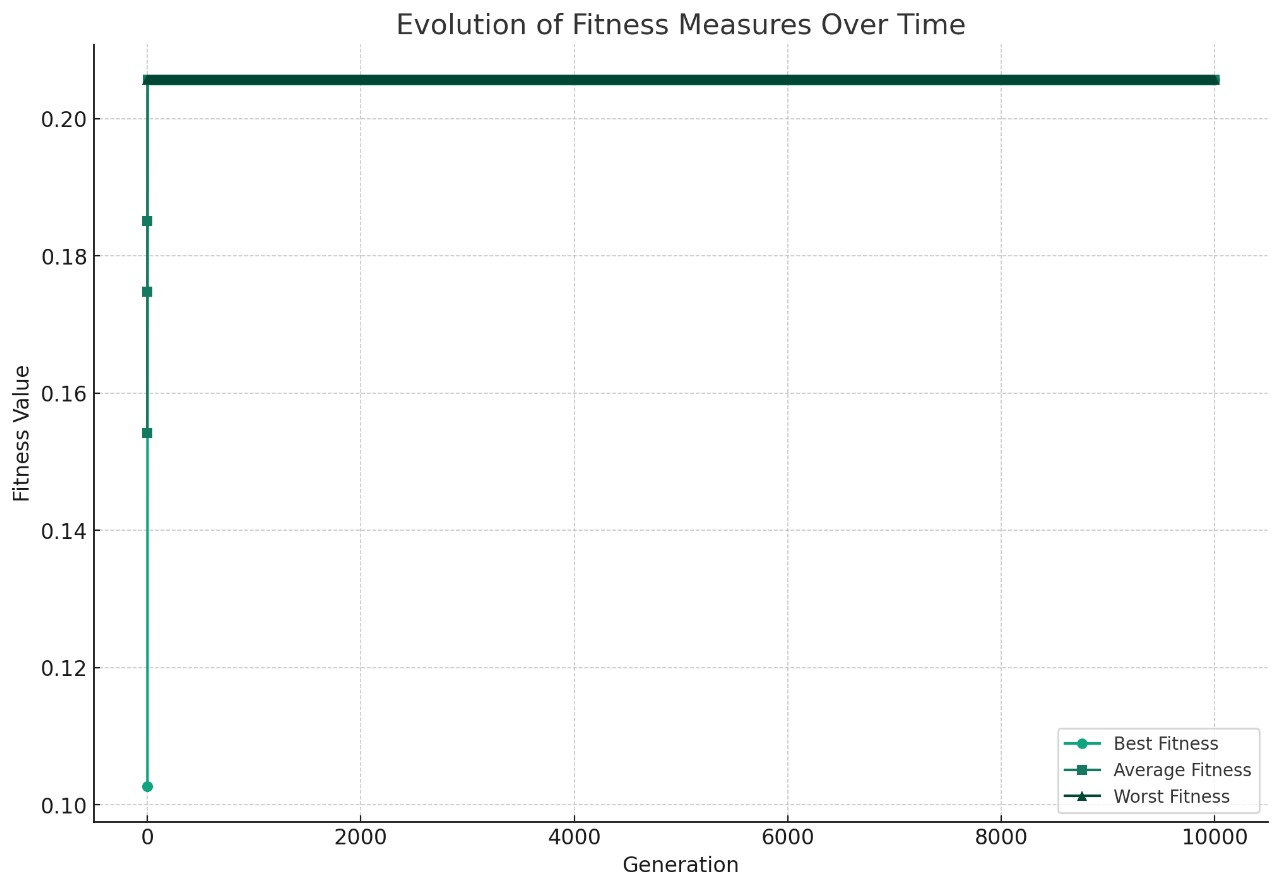
\includegraphics[width=0.5\linewidth]{1tentativa.png}
    \caption{Evolução da população com 10000 gerações}
    \label{fig:first-attempt}
\end{figure}

No teste seguinte a mudança  foi aplicada ao número de gerações com 200(2(\%da primeira tentativa) e obteve-se resultados melhores, porém com pouca informação para ser analisada.

\begin{figure}[h]
    \centering
    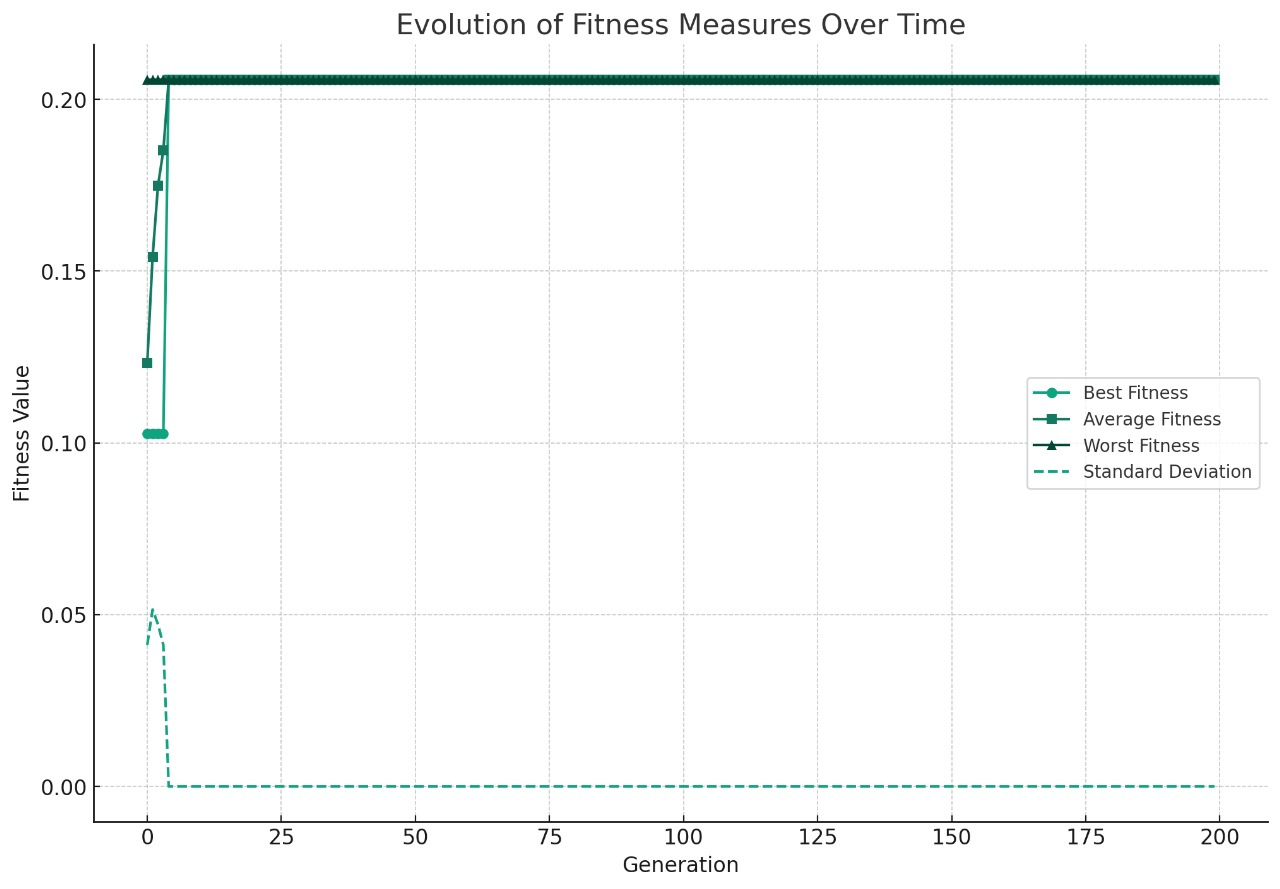
\includegraphics[width=0.5\linewidth]{2tentativa.png}
    \caption{Evolução da população com 200 gerações}
    \label{fig: second-attempt}
\end{figure}

Na terceira tentativa, ambos número de gerações e número de da população foram mudadas para 100, e com isso resultados mais satisfatórios foram apresentados.

\begin{figure}[H]
    \centering
    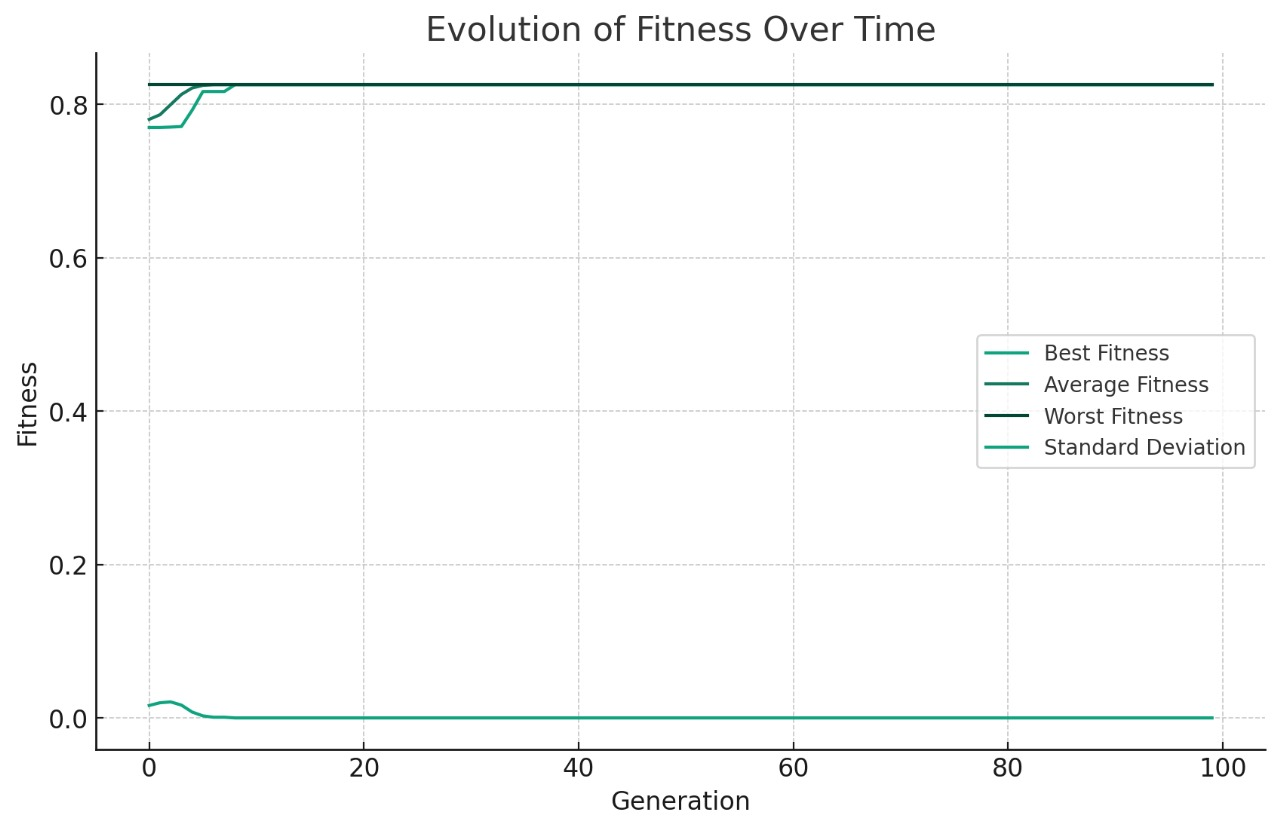
\includegraphics[width=0.5\linewidth]{3tentativa.png}
    \caption{Evolução da população com 100 gerações e 100 indivíduos}
    \label{fig:third-attempt}
\end{figure}

Na última tentativa com a população agora com o tamanho de 1000, o tempo de processamento aumentou significativamente porém os resultados quase não mudaram. Com um desvio padrão de aproximadamente de 0.01 e fitness entre 0.76 e 0.84

\begin{figure}[h]
    \centering
    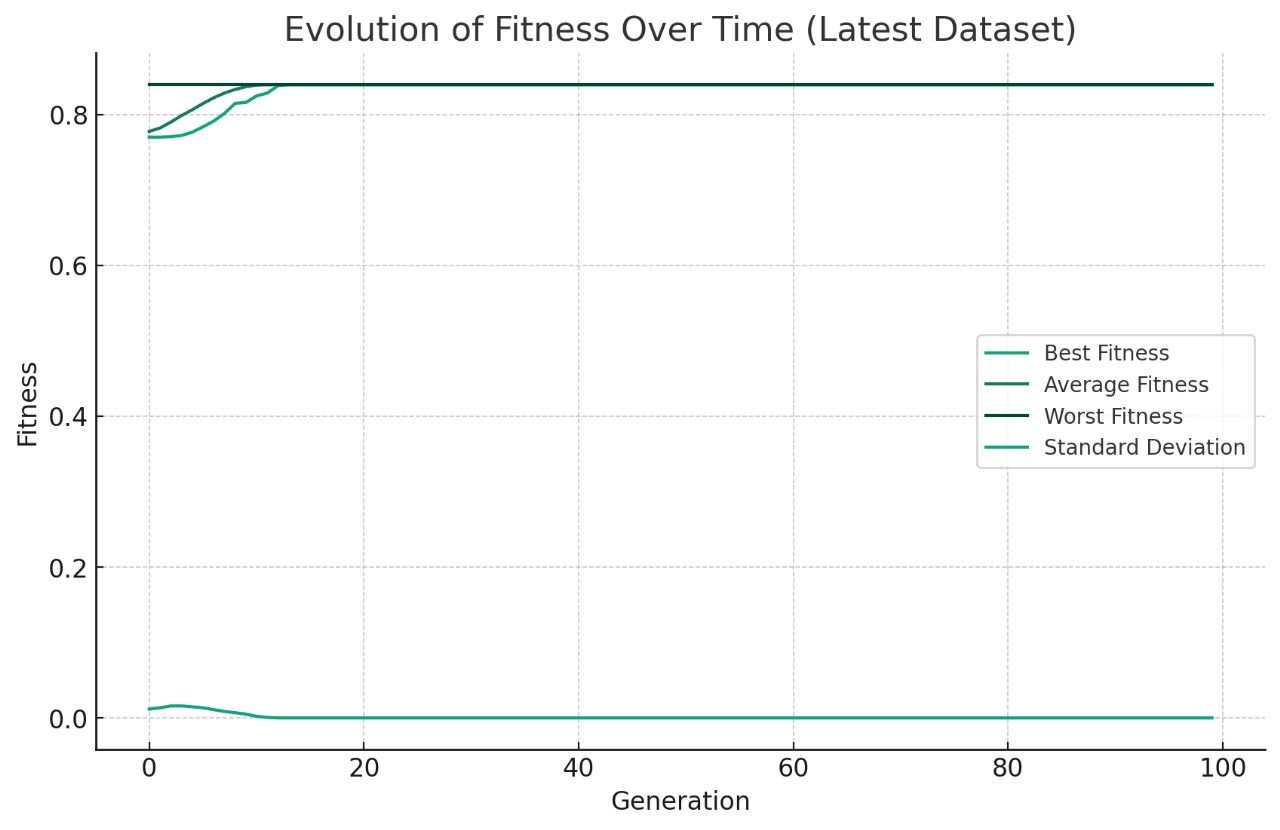
\includegraphics[width=0.5\linewidth]{4tentativa.png}
    \caption{Evolução da população com 100 gerações e 1000 indivíduos}
    \label{fig:fourth-attempt}
\end{figure}

\section{Conclusões}
Afim de diminuir as consequências negativas de incêndios e em conclusão do que foi escrito nesse papel, dado que entre os fatores que foram analisados há três tipo de vegatação, três estados de propragação do fogo, a umidade do ar.
Depois de todos os testes o resultado final obtido foi com a população com tamanho 1000 e 100 iterações, porém com aproximadamente apenas 16 iterações resultou num ótimo de aproximadamente 0.99, o que significa que o algoritmo proposto teve 99\% de compatibilidade com a simulação real, resultado notável para auxiliar no combates a incêndios.

\section{References}


\bibliographystyle{sbc}
\bibliography{mybib}

\end{document}
